\documentclass[a4paper,12pt]{article}
\usepackage[utf8]{inputenc}
% \usepackage{fontspec}
% \usepackage[spanish]{babel}
\usepackage{graphicx}
\usepackage{hyperref}
\usepackage{amssymb, gensymb}
\usepackage{amsmath, mathtools}

\title{Manual de Usuario de Stack Calculator}
\author{Ian Logan Will Quispe Ventura}
\date{ }
\begin{document}

\maketitle
% \tableofcontents
% \newpage

\section{Introducción}
\underline{waw}
El programa de calculadora "Stack Calculator", es una calculadora basada en el manejo de pila y expresiones posfijas, el funcionamiento básico es el siguiente.

El programa recibe las operaciones y estas se calculan a traves de una pila, luego el resultado es mostrado en la calculadora. 

\section{Características}
Características resaltantes de la calculadora.
\begin{itemize}
    \item Soporte de operaciones de suma, resta, multiplicación, división y potenciación.
    \item Soporte de expresiones aritméticas respetando las prioridades de las operaciones y símbolos de agrupación.
    \item Soporte de las acciones Deshacer y Rehacer en la edición de la expresión aritmética ingresada.
    \item Soporte de inserción y edición de las expreiones matemáticas desde el teclado 
    \item Interfaz gráfica simple, clara y sencilla de usar.
\end{itemize}

\section{Descripción de la Interfáz gráfica}
La calculadora se ve de la siguiente manera.
%%%
\begin{figure}[h!]
    \centering
    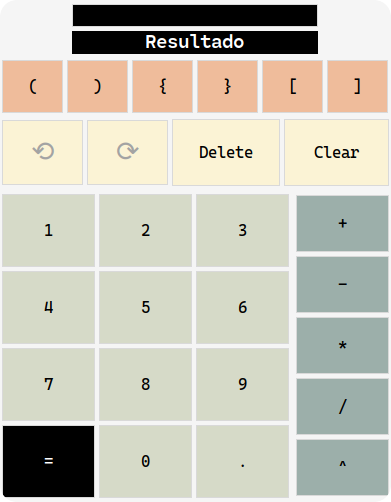
\includegraphics[width=0.7\textwidth]{../img/calculator1.png}
    \caption{Vista frontal de la calculadora}
    \label{fig:vista-frontal}
\end{figure}

A continuación revisaremos y explicaremos cada elemento de la interfaz de la calculadora. 
\subsection{Pantallas de entrada y salida}
En la parte superior de la aplicación se puede encontrar 2 pantallas.
\begin{itemize}
    \item Pantalla de edición e incersión de las expresiones aritméticas.
    \item Pantalla de resultado, no es editable. 
\end{itemize}

\subsection{Botones}
Inmediatamente despues de las pantallas encontraremos los botones que servirán para introducir y editar las expresiones aritméticas y para calcular el resultado correspondiente. 
\subsubsection{Símbolos de agrupación}
Estos símbolos permiten delimitar las operaciones dentro de una expresión aritmpetica. Estas son: 

\begin{figure}[h!]
    \centering
    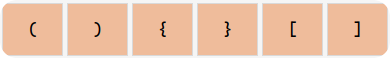
\includegraphics[width=0.6\textwidth]{../img/agrupacion.png}
    \caption{Símbolos de agrupacion}
    \label{fig: agru}
\end{figure}
\begin{itemize}
    \item \textbf{(} Símbolo de apertura de paréntesis
    \item \textbf{)} Símbolo de cerradura de paréntesis
    \item \textbf{\{} Símbolo de apertura de llave 
    \item \textbf{\}} Símbolo de cerradura de llave
    \item \textbf{[} Símbolo de apertura de corchete
    \item \textbf{]} Símbolo de cerradura de corchete
\end{itemize}
\subsubsection{Botones de acción}
Estos botones permiten manejar la edición de la expresión aritmética, estos son:
\begin{figure}[h!]
    \centering
    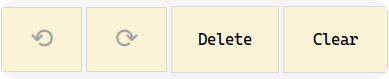
\includegraphics[width=0.6\textwidth]{../img/acciones.png}
    \caption{Botones de acción}
    \label{fig: accioens}
\end{figure}
\begin{itemize}
    \item \textbf{$\circlearrowleft$} Símbolo de deshacer, este botón se habilita solo cuando haya operaciones disponibles.
    \item \textbf{$\circlearrowright$} Símbolo de rehacer, este botón se habilita solo cuando haya operaciones disponibles.
    \item \textbf{Delete} Eliminar el último elemento de la expresión
    \item \textbf{Clear} Limpiar las de inserción y de resultado.
\end{itemize}

\subsubsection{Números}
Los botones de los números del 0 al 9 están estructurados en una matriz 3x3, donde además, se añade el boton de punto decimal y el boton igual.
\begin{figure}[h!]
    \centering
    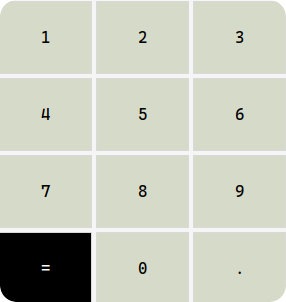
\includegraphics[width=0.5\textwidth]{../img/botones.png}
    \caption{Botones de numeración}
    \label{fig: botones}
\end{figure}
\subsubsection{Operaciones}
\begin{figure}[h!]
    \centering
    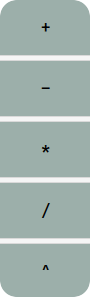
\includegraphics[width=0.13\textwidth]{../img/operaciones.png}
    \caption{Botones de numeración}
    \label{fig: operaciones}
\end{figure}
Los botones de operaciones están organizados en una columna a la derecha de la aplicación, las operaciones disponibles son:
\begin{itemize}
    \item \textbf{+} símbolo de la operación suma 
    \item \textbf{-} símbolo de la operación resta
    \item \textbf{*} símbolo de la operación multiplicación 
    \item \textbf{/} símbolo de la operación división 
    \item \textbf{\^} símbolo de la operación potenciación 
\end{itemize}

\subsubsection{Botón de resultado}
El botón '\textbf{=}' permite calcular el resultado de la expresión aritmética ingresada, esto se hará usando la logica de la aplicación en base a pila.

\section{Instrucciones de Uso}
\subsection{Ejecutar el programa}
Para ejecutar el programa solo hace falta dar dos veces click en el ícono de la aplicación, que es 'Stack Calculator', No es necesario instalar ninguna dependencia.

\subsection{Ingresar y editar las expresiones aritméticas}
Una vez iniciado el programa podremos ingresar la expresión aritmética oprimiendo los botones deseados, o usando el teclado.

El programa solo permite que se añadan los números, símbolos y operaciones que se muestran en los botones, por lo que no se añadirán letras ni otros símbolos ajenos al programa.

Recuerda que también tenemos los botones de acción, estos botones los usaremos para deshacer, rehacer las acciones echas en la expresión aritmética.

Con botón Delete eliminaremos el último elemento de la expresión y lo añade a la pila de Redo, por lo que podrémos recuperarlo haciendo click en el botón de rehacer. 

Con el botón Clear limpiamos las pantallas y las pilas del programa.

\subsubsection{Calcular el resultado}
Calcular el resultado se hace simplemente oprimiendo el botón \textbf{=} o presionando la tecla 'Enter' del teclado físico.


\subsection{Errores}
\subsubsection{Expresión no balanceada}
\begin{figure}[h!]
    \centering
    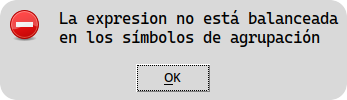
\includegraphics[width=0.5\textwidth]{../img/error2.png}
    \caption{Botones de numeración}
    \label{fig: no balanceada}
\end{figure}
Este error se da cuando la expresión tiene símbolos de agrupación que no están balanceados, algunos ejemplos de expresiones que generan este error son.
\begin{itemize}
    \item \textbf{123+(} 
    \item \textbf{ [11+\{12(*12] }
    \item \textbf{\{24*78]\}}
    \item \textbf{ [\{(12+3) }
\end{itemize}
Si se intenta calcular el resultado de una expresión no balanceda, emergerá una ventana que muestrará error respectivo, para salir de ella debemos simplemente dar click en 'Aceptar' o 'Ok' dependiendo el lenguaje del sistema.

\subsubsection{Exresión incorrecta}
\begin{figure}[h!]
    \centering
    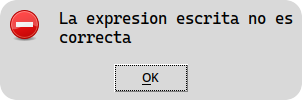
\includegraphics[width=0.5\textwidth]{../img/error1.png}
    \caption{Botones de numeración}
    \label{fig: inconsistente}
\end{figure}
Este error se da cuando la expresión matemática contiene inconsistencias más allá de los símbolos de agrupamiento, estos puedes ser los siguientes.
\begin{itemize}
    \item \textbf{123++} 
    \item \textbf{ 11+*12 }
    \item \textbf{12+()}
    \item \textbf{ +12-1* }
\end{itemize}
Si se intenta calcular el resultado de una expresión no balanceda, emergerá una ventana que muestrará error respectivo, para salir de ella debemos simplemente dar click en 'Aceptar' o 'Ok' dependiendo el lenguaje del sistema.


\section{Funcionamiento explícito del programa}
Esta es una calculadora a base de pilas, por lo que todo girará en torno a ellas.
Una vez ingresada la expresión en la pantalla de inserción, se habilitarán los botones de deshacer y rehacer debido a que se almacenaron los elementos introducidos en las pilas correspondientes.

Si estas pilas se vacián entonces los botones quedarán desabilitados, pues no hay operaciones a realizar.\\

Al momento de calcular un expresión, primero se verificará si es que la expresión es consistente, a través de 'expreiones regulares', cada posible inconsistencia está contenidad en el procesp de verificación, si la expresión es incorrecta entonces no se procesa el resultado y se informa sobre el error. 

Si la expresión es consistente entonces se pasará al proceso de verificación del balanceo. Este proceso se realiza usando expreiones regularesy pilas, cuando se encuentre un símbolo de apertura, este se añadirá a la pila, cuando se encuentre su respectivo elemento de cerradura, entonces el simbolo inicial se desapilará, de tal manera, que si una expresión está balanceada la pila también lo estará. Si no es así, entonces no se completará el cáclulo de la expresión y se informará sobre el error.

Si la expresión está balanceada entonces se iniciará el proceso para transformar la expresión infija a posfija, a este proceso se le llama comunmente 'parsear' o 'tokenizar'. Cada elemento de la expresión será añadido a una pila donde posteriormente se calculará el resultado.

Finalmente podemos calcular el resultado, tenemos una pila llena de elementos de una expresión aritmética. Accederemos a los dós elemento de arriba de la pila, los operaremos y el resultado lo debolveremos a la pila y volveremos a hacer este proceso hasta teminar con todos los elementos. Nos quedará un punico elemento en la pila, este es el resultado y será mostrado en la pantalla de resultado. 
\end{document}

